\documentclass[twocolumn,linenumbers]{aastex631}

% Packages
\usepackage{microtype}  % ALWAYS!
\usepackage{amsmath}
\usepackage{amsfonts}
\usepackage{amssymb}
\usepackage{multirow}
\usepackage{tikz}
\usepackage{xcolor}
\usepackage{soul}

% defining colors for personalized comments
\definecolor{pink}{RGB}{232,132,161}
\definecolor{yellow}{RGB}{255,213,0}
\newcommand{\kc}[1]{\textcolor{yellow}{\textbf{kc: #1}} }
\newcommand{\ep}[1]{\textcolor{pink}{\textbf{e: #1}} }

% defining affiliations
\newcommand{\affuofa}{University of Arizona, 933 N. Cherry Ave,
    Tucson, AZ 85721, USA}
\newcommand{\affuofu}{Department of Astronomy, University of Utah, Salt Lake City, UT 84112, USA}

% reference to previous paper
\newcommand{\chambe}{\citet{Chamberlain2024}}

% Style tweaks
\sloppy\sloppypar\raggedbottom\frenchspacing

% Inputs for path to plots and math defs
\graphicspath{{./}{../plots/}}
% Missions
\newcommand{\project}[1]{\textsl{#1}}

% Packages / projects / programming
\newcommand{\package}[1]{\textsl{#1}}
\newcommand{\acronym}[1]{{\small{#1}}}
\newcommand{\github}{\package{GitHub}}
\newcommand{\python}{\package{Python}}
\newcommand{\astropy}{\package{Astropy}}

% Stats / probability
\newcommand{\given}{\,|\,}
\newcommand{\norm}{\mathcal{N}}
\newcommand{\pdf}{\textsl{pdf}}

% Maths
\newcommand{\dd}{\mathrm{d}}
\newcommand{\transpose}[1]{{#1}^{\mathsf{T}}}
\newcommand{\inverse}[1]{{#1}^{-1}}
\newcommand{\argmin}{\operatornamewithlimits{argmin}}
\newcommand{\mean}[1]{\left< #1 \right>}

% Non-scalar variables
\renewcommand{\vec}[1]{\ensuremath{\bs{#1}}}
\newcommand{\mat}[1]{\ensuremath{\mathbf{#1}}}

% Unit shortcuts
\newcommand{\Msun}{\ensuremath{\mathrm{M}_\odot}}
\newcommand{\Mjup}{\ensuremath{\mathrm{M}_{\mathrm{J}}}}
\newcommand{\kms}{\ensuremath{\mathrm{km}~\mathrm{s}^{-1}}}
\newcommand{\pc}{\ensuremath{\mathrm{pc}}}
\newcommand{\kpc}{\ensuremath{\mathrm{\,kpc}}}
\newcommand{\Mpc}{\ensuremath{\mathrm{Mpc}}}
\newcommand{\kmskpc}{\ensuremath{\mathrm{km}~\mathrm{s}^{-1}~\mathrm{kpc}^{-1}}}
\newcommand{\dayd}{\ensuremath{\mathrm{d}}}
\newcommand{\yr}{\ensuremath{\mathrm{yr}}}
\newcommand{\Myr}{\ensuremath{\mathrm{Myr}}}
\newcommand{\Gyr}{\ensuremath{\mathrm{\,Gyr}}}
\newcommand{\Kel}{\ensuremath{\mathrm{K}}}
\newcommand{\masyr}{\ensuremath{\mathrm{mas}~\mathrm{yr}^{-1}}}
\newcommand{\muasyr}{\ensuremath{\mu\mathrm{as}~\mathrm{yr}^{-1}}}

% Misc.
\newcommand{\bs}[1]{\boldsymbol{#1}}

% Astronomy
\newcommand{\DM}{{\rm DM}}
\newcommand{\feh}{\ensuremath{{[{\rm Fe}/{\rm H}]}}}
\newcommand{\df}{\acronym{DF}}

% TO DO
\newcommand{\todo}[1]{{\color{red} TODO: #1}}
\newcommand{\apw}[1]{{\color{blue} APW says: #1}}

% Projects
\newcommand{\gaia}{\textsl{Gaia}}
\newcommand{\gaiadr}{\textsl{Gaia}~\acronym{EDR3}}
\newcommand{\hst}{\textsl{HST}}

% Paper specific
\newcommand{\paircat}{\textit{Full Pair Catalog}}

\newcommand{\lcdm}{\ensuremath{\Lambda \rm CDM}} 
\newcommand{\sublink}{\textsc{sublink}} 
\newcommand{\subfind}{\textsc{subfind}} 

% masses - halo
\newcommand{\Mpeak}{\ensuremath{M_{\mathrm{peak}}}}
\newcommand{\Mhalo}{\ensuremath{M_{\mathrm{h}}}}
\newcommand{\MG}{\ensuremath{\rm M_{\mathrm{G}}}}
\newcommand{\mlg}{\ensuremath{M_{\rm LG}}}

% masses - stellar
\newcommand{\Ms}{\ensuremath{\rm M_{{*}}}}
\newcommand{\msam}{\ensuremath{M_{*,\mathrm{am}}}}
\newcommand{\mssim}{\ensuremath{M_{*,\mathrm{sim}}}}
\newcommand{\ms}[1]{\ensuremath{M_{*{#1}}}}

\newcommand{\vtan}{\ensuremath{v_\textrm{tan}}}
\newcommand{\vrad}{\ensuremath{v_\textrm{rad}}}
\newcommand{\reflabel}[1]{\ensuremath{^{\mbox{\scriptsize{#1}}}}}

\newcommand{\Rvir}{\ensuremath{\rm R_{vir}}}
\newcommand{\Rphys}{\ensuremath{\rm R_{phys}}}
\newcommand{\Rsc}{\ensuremath{\rm R_{sc}}}
\newcommand{\rsep}{\ensuremath{\rm r_{sep}}}

%%%%%%%%%%%%%%%%%%%%%%%%%%%%%%%%%%%%%%%%%%%%%%%%%%%%%%%%%%%%%%%%%%%%%%%%%%%%%%%%
\begin{document}

\title{A Physically Motivated Framework to Compare Merger Timescales\\ of Isolated Low- and High-Mass Galaxy Pairs Across Cosmic Time
}
\shorttitle{Merger Timescales in TNG100}

\author[0000-0001-8765-8670]{Katie~Chamberlain}
\affiliation{\affuofa}

\author[0000-0002-9820-1219]{Ekta~Patel}
\thanks{Hubble Fellow}\affiliation{\affuofu}

\author[0000-0003-0715-2173]{Gurtina Besla}
\affiliation{\affuofa}

\author{others}

\shortauthors{Chamberlain et al.}


\begin{abstract}
    % Statement
    % Evolutionary differences between low-mass ($\rm 10^8<M_*<5\times10^9\,\Msun$) and high-mass ($\rm 5\times10^9<M_*<10^{11}\,\Msun$) galaxy pairs have been studied in detail for the last few decades, with studies finding differences in star formation rates, gas fractions, and dark matter halo profiles. % could remove this line 
    % Problem 
    The merger rates of high-mass pairs ($\rm 5\times10^9<M_*<10^{11}\,\Msun$) have been studied extensively, both observationally and theoretically. 
    Since low-mass pairs ($\rm 10^8<M_*<5\times10^9\,\Msun$) are comparatively under studied, it is common to apply the same separation criteria and expected merger timescales of high-mass pairs to low-mass systems.
    However, it is unclear if using the same separation criteria to select low-mass galaxy pairs for such studies, or if using the same separation criteria at different redshifts, permits an equitable comparison between galaxies of different mass and redshift. 
    % Our solution
    Here, we present a physically-motivated framework by which merger timescales for high-mass and low-mass pairs can be compared equivalently, 
    %and converted from one system to another 
    %by scaling 
    % GB added below
    wherein separation criteria are scaled
    by the virial radius of the primary's FoF group halo ($r_{\mathrm{sep}}< 1 R_{\rm vir}$). 
    We use the Illustris TNG100 simulation to quantify the merger timescales of isolated low-mass major pairs as a function of cosmic time, and compare to the merger timescales of similarly-selected high-mass major pairs. 
    Using our framework to select pairs via a scaled separation criterion leads to equivalent merger timescales for low- and high-mass systems at redshifts $z=0-6$. 
    % What are the timescales? 
    Alternatively, static physical separation selections applied equivalently to all galaxy pairs at all redshifts, particularly for the closest pairs ($\rsep<150\kpc$), leads to timescales that differ by up to $\sim1\Gyr$ between low- and high-mass pairs. 
    % Why it matters 
    Our findings suggest that the comparison of low-mass and high-mass galaxy pair fractions, merger timescales, and merger rates is self-consistent using separation criteria that scales as a function of mass and redshift of the system. 
    As a result, applying the same merger timescales to different mass systems will lead to a bias that systematically (over/under) predicts low-mass galaxy merger rates. 
\end{abstract}
%%%%%%%%%%%%%%%%%%%%%%%%%%%%%%%%%%%%%%%%%%%%%%%%%%%%%%%%%%%%%%%%%%%%%%%%%%%%%%%%


%%%%%%%%%%%%%%%%%%%%%%%%%%%%%%%%%%%
\section{Introduction} \label{sec:intro}
Outline draft - 
1 - Galaxy mergers are an importance feature of LCDM theory and are critical for the formation and evolution of galaxies across time. 
    - An important feature of galaxy mergers is the merger timescale...

2 - Merger timescales are important to calibrate 
    - They are crucial for understanding the observations of galaxy morphologies and understanding heirarchical evolution, (think galaxy start bursts, formation of gas bridges maybe, fueling agn, BH merger rates, etc)
    - Also important for understanding the few well modelled orbits that we do have, particularly in the LG (might come way later) 

3 - Merger timescales are also used to get merger rates, both observationally and theoretically, of close pairs.
    - How are close pairs defined? 
    - How do merger timescales enter merger rate calculations?
    - What is important about the merger rates that are used? 
    - Maybe need to make distinction here that there are also observability timescales, but they are going to be basically useless for TNG100 studies (see below), but also are low mass pairs have a lot of gas and look super weird. 
    - RG 2019 looked at the simulated morphology of illustristng galaxies and found that for $M*<1e9.5$, the morphologies are "less reliable" $\to$ motivates using pair fractions for merger rate studies 


4 - Comparing the merger rates of high mass and low mass pairs is important why?
    - Is important for our understanding of the build up of higher mass things in LCDM, and thus a test of LCDM
    - Different merger mechanics would be really interesting, i.e. if the DM halo profile (cuspy/core etc) impacted the merger processes

5 - Merger timescales have been studied a lot (mostly in obs and theory of high mass pairs)
    - Lotz 2011
    - RG2015
    - Snyder (maybe?) 
    - Jiang 2008 \& BK 2008 for all things about the "Chandra" timescale for merging galaxies which scales with rc/Vc and is thus prop to the age of the universe (eq. 4\&5). Also quantified the circularity of orbits as a function of mass ratio $\leftarrow$ might be good to mention
    - Jiang 2014 

6 - Problem is, we don't have a lot of studies on low mass pair merger rates? 
    - This is not ideal because it means that we typically extend merger rates calibrated for high mass down to low mass, but this means that we aren't able to test LCDM and draw conclusions about the impact

7 - In addition, our previous work showed that even the evolution of the fractions of high and low mass pairs can't be robustly studied and compared if even the selection criteria for the pairs are off. 
    - This means that the selection of pairs for pair fractions, merger fractions, and for merger timescales, are ALL going to be impacted by the selection criteria that's used. 
    - This is also a problem in observations already, since different samples will have different completeness down to different projected separations, and with different mass ratios, etc. 
    - O'Leary 2021 merging systems can be missed if you don't use wide enough sep criteria, thus leading to under predict merger rate

8 - Fortunately, our previous work showed that using scaled criteria for pair selection as a function of mass and redshift allows you to fairly compare samples. 
    - This motivated us to study the merger fraction and merger timescales of our galaxy pair sample from the first study, to see how merger timescales might ALSO depend on the selection criteria that are used to pick the pair sample. 


9 - Here, we aim to build a framework to understand the pair selection criteria that are used to select samples, and the merger timescales that result from various selections.  we look at the orbits of the pairs from our previous work, and determine the merger timescale for low and high mass pairs as a function of pair separation and redshift. In sec. 1... etc. 

%%% OUTLINE
\section{Methodology} \label{sec:methods}
%recap last paper and mention which data sample we narrow down to (low mass major pairs only) -- give examples of orbits
We utilize the group catalogs, produced by the \subfind{} algorithm~\citep{Springel2001b,Dolag2009}, and the merger tree catalogs, generated by the \sublink{} algorithm~\citep{RG2015}, from the highest resolution run of the IllustrisTNG simulation TNG100-1 (hereafter TNG100) to study the merger timescales of galaxy pairs from $z=0-6$.
The catalogs consist of a set of 100 snapshots, ranging from $z\sim20$ (snapshot 0) to $z=0$ (snapshot 99).

Our sample consists of major (stellar mass ratio $M_{*2}/M_{*1}= 1/4 - 1$) low-mass and high-mass pairs that are isolated, but physically associated, as in \citet{Chamberlain2024}.
From this sample, we will determine the fraction of pairs at each snapshot that merge before $z=0$, and track the orbits of each pair to study their merger timescales.

\subsection{Pair sample}
We begin with an extension of the \paircat{} described in \chambe{}, which consists of a collection of isolated galaxy pairs at each snapshot in TNG100. 
We collect our base sample at each redshift in the simulation. 
A brief version of the selection routine is transcribed here for completeness, and we refer readers to Sec.~2 of \chambe{} for more detail and a discussion of the selection criteria choices. 

At each snapshot, low-mass and high-mass pairs are chosen by first selecting the two most massive subhalos (by assigned stellar mass, using abundance matching; see below) from FoF groups with virial mass 
% GB added M_G
($\rm M_{G}$)\footnote{We use \texttt{Group\_M\_TopHat200} from the TNG100 Group Catalogs as the FoF Group virial mass. This mass is defined to be the mass enclosed by a sphere with mean density $\Delta_c *\rho_c$, where $\Delta_c$ is the overdensity constant from~\citet{Bryan1998} and $\rho_c$ is the critical density of the universe at the time calculated. The corresponding virial radius in TNG100 is given by \texttt{Group\_R\_TopHat200}.} 
\begin{align*}
        \mbox{\textbf{low mass:}}&\,\rm M_{G} = 8\times 10^{10}- 5\times 10^{11}\,\Msun \\ 
        \mbox{\textbf{high mass:}}&\, \rm M_{G}=1\times 10^{12}- 6.5\times10^{12}\,\Msun.
\end{align*}
Utilizing the most massive subhalos from the same FoF group ensures that the pairs are isolated from other massive nearby systems that could perturb the dynamical state of the pair. 

We require that subhalos constituting a pair meet a minimum subhalo mass 
% GB added Mhalo
($\Mhalo$)
criteria of 
\begin{equation*}
    \mbox{\textbf{minimum subhalo mass:}}\,
    \Mhalo > 1\times10^{9}\Msun.
\end{equation*}
at the snapshot of consideration. 
For TNG100, this ensures that subhalos are resolved into over 
$\sim$100 particles, enough to robustly identify gravitationally bound subhalos in the \subfind{} and \sublink{} catalogs.
For each subhalo in the FoF group that passes the minimum subhalo mass criteria, we utilize the \sublink{} catalogs to find the peak halo mass of each subhalo \citep{RG2015}. 

% GB added 
As in \chambe{}, 
stellar masses are assigned to each subhalo in the FoF group using the abundance matching prescription of \citet{Moster2013}. 
The peak halo mass and current redshift are used to calculate the stellar mass of each subhalo via the abundance matching prescription  $\ms{}=f(\Mpeak,z)$, where $z$ is the redshift of consideration.

In \chambe{}, 
abundance matching prescription was sampled 1000 times for each subhalo to account for the spread in the Stellar Mass -- Halo Mass (SMHM) relation. 
For the present study, we only use the stellar masses given by the median of the abundance matching relationship. 
We expect that the spread of merger timescales from different orbital configurations, as well as the redshift spacing of the TNG100 snapshots, will dominate over uncertainties from the number of pairs in the catalog, which varied by $\sim3\%$ (as shown in Fig.~1 in \chambe{}). 
% Since we will be following the orbits of selected pairs both backwards and forwards in time, the 

Primary subhalos are defined as the subhalo with the highest assigned stellar mass ($M_{*1}$) in their FoF group, and secondaries are defined as the second most massive subhalo with stellar mass $M_{*2}$. 
Our sample of major pairs then consists of all pairs of primary and secondary subhalos with 
\begin{align*} 
\mbox{\textbf{low mass primaries:}}&\, 10^{8}< \rm M_{*1} < 5\times10^{9} \Msun \\ 
\mbox{\textbf{high mass primaries:}}&\, 5\times 10^{9}< \rm M_{*1} < 10^{11} \Msun\\
\mbox{\textbf{stellar mass ratio:}}&\,      
    M_{*2}/M_{*1} > 1/4.
\end{align*}
A primary or secondary subhalo can only be a member of one single pair at a given snapshot, such that a collection of $N$ pairs consists of $N$ unique primaries and $N$ unique secondaries.

A subhalo can belong to different pairs at different redshifts. 
For example, the primary of a pair that merges at $z=2$ can be selected with a different secondary at $z=1$, constituting a new pair. 
More detail regarding the uniqueness of pairs and orbits is discussed in~\ref{sec:methods-unique}.

% I removed the 10kpc component of this because I think it'd just be easier to handle those cases in the results sections or orbits section
% Finally, we will only consider pairs that have physical separations of $\rsep>10\,\kpc$ at the snapshot of selection. 
% The physical separation cut does not vary with redshift, and is the same for both low-mass and high-mass pairs. 

The base sample of pairs used for this analysis then consists of the set of all
% GB added
isolated 
low-mass and high-mass major pairs from each redshift of the TNG100 simulation. 

\subsection{Mergers} \label{subsec:mergers}
Here we describe how subhalo mergers are identified. 
Note that this definition is specific to subhalo mergers and therefore results are not guaranteed to hold for galaxy mergers, especially in cases where subhalos and galaxies have different centers of mass~\citep[see e.g.,]{RG2015}. % might  note that this is discussed in more deets in discussion - I think Patton 2024 addresses this a bit?
The primary and secondary subhalos of each pair have a `SubfindID' that is used to identify them in the \subfind{} merger tree catalogs, which contain information about every FoF group and subhalo at each redshift. 
The \sublink{} catalogs track subhalos from one redshift to the next, and thus enable us to track subhalos both backwards and forwards in time from any given redshift. 

We utilize the \texttt{DescendantID} field of the \sublink{} catalogs to determine which pairs from our base sample merge before the end of the simulation (at $z=0$) and when the merger occurs. 
The \texttt{DescendantID} field provides the `SubhaloID'\footnote{Note that the `SubhaloID' is distinct from the `SubfindID', and is unique for every subhalo in the merger trees. 
The \sublink{} catalogs provide the associated `SubfindID' of each subhalo.} of the subhalo's descendent in the next (or one of the following) snapshots, if it has one. 

In this analysis, a pair is classified as a merger if the primary and secondary subhalo share the same \texttt{DescendantID} at the same redshift. 
This means that the primary and secondary subhalo have merged such that \subfind{} can no longer distinguish them as two separate halos, therefore yielding a single descendant subhalo.
If a primary and secondary never share the same \texttt{DescendantID} at the same redshift, the pair is defined as a `non-merger.'

For each merging pair, we define the `merger redshift' as the redshift that immediately follows the first snapshot where the primary and secondary have the same \texttt{DescendantID}. 
For example, if the primary and secondary have different \texttt{DescendantIDs} from $z=6$ to $z=2$, but have the same \texttt{DescendantID} at $z=2$, then the merger must take place some time between $z=2$ and $z=1.9$, which is the next redshift corresponding to a snapshot in the simulation. 
In this example, we take $z=1.9$ to be the merger redshift. 

\subsection{Orbits} 
\begin{figure}[tb]
    \begin{center}
    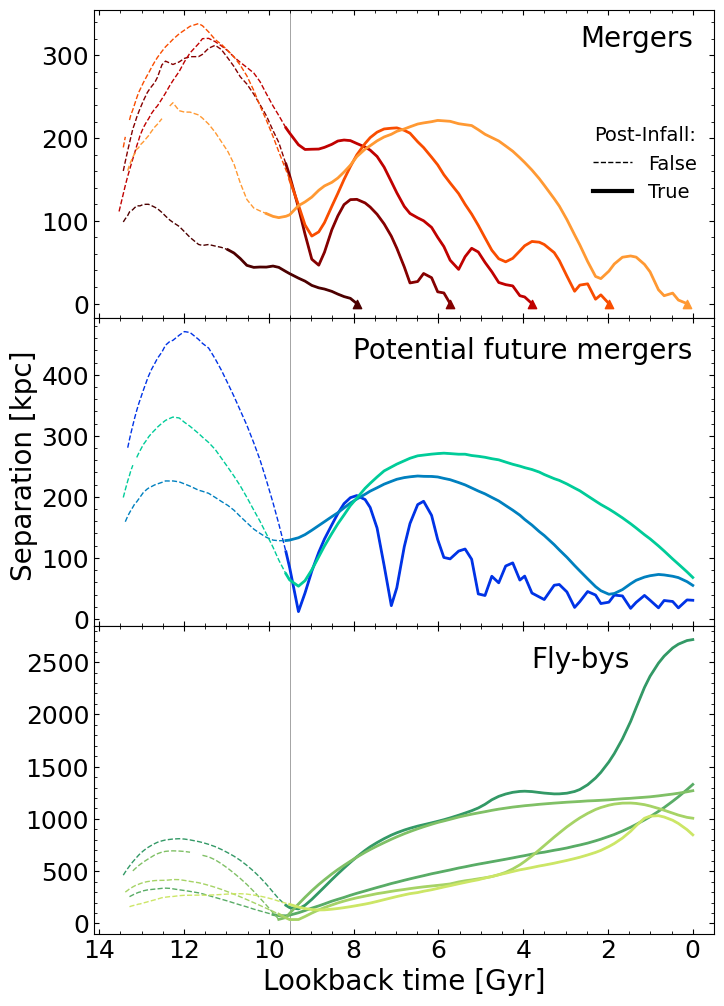
\includegraphics[width=\columnwidth]{plots/bet-on-it/5_exampleorbits.png}
    \caption{Selection of example orbits of low-mass major pairs that pass the pair selection criteria at $z=1.5$, showing the separation between the primary and secondary as a function of lookback time. 
    (Top) Orbits of pairs that merge before $z=0$.
    (Middle) Orbits of pairs that do not merge before $z=0$ (non-mergers), but are likely to merge if the simulation continued. 
    (Bottom) Orbits of pairs that do not merge before $z=0$ (non-mergers) and are unlikely to do so in the future $\sim2\Gyr$ (past the end of the simulation).
    Solid lines represent the post-infall orbits, i.e. after the pair share a common FoF group.
    Dashed lines show the pre-infall portion of the orbit. 
    Triangle points in the first panel show the first redshift after merger where the orbit has a separation of $0\,\kpc$.
    The vertical grey line marks $z=1.5$ at a lookback time of $9.5\,\Gyr$. 
    }
    \label{fig:example-orbits}
    \end{center}
\end{figure}

We extract orbits for all mergers and non-mergers in our base pair sample. 
An orbit for a single pair is defined to be the physical separation between the primary and secondary subhalo as a function of redshift (or lookback time). 

A given pair from the base sample at redshift $z_n$ passes all of the selection criteria from \chambe{} at $z_n$, and can additionally be followed backwards and forwards in time using the \sublink{} merger trees. 
We track the positions of both the primary and secondary subhalo at each redshift and calculate the physical separations after accounting for the periodic boundary conditions of the simulation box.
In cases where the primary or secondary does not have a defined position at a given redshift, we do not compute a value for the separation at that redshift.\footnote{If a subhalo is very small, or is passing through a more massive subhalo, and is unable to reach the density contrast required to be identified as an independent structure by the \subfind{} algorithm, it will not have a defined position in the \sublink{} catalogs. The \sublink{} algorithm allows for subhalos to skip a single snapshot, and identifies the `skipped descendent' in the $S_{n+2}$ snapshot, so that the orbit can be evaluated before and after the skip occurs. See Sec.~3 in ~\citet{RG2015} for more details.}

In addition to the physical separation, we also calculate the scaled separation of a pair at each redshift. We use the definition of scaled separation from~\cite{Chamberlain2024}, where the physical separation is written instead as a fraction, $p$, of the virial radius $\rsep=p\Rvir$, where $\rsep$ is the physical separation in $\kpc$, and $\Rvir$ is the virial radius of the pair's FoF group (also in $\kpc$).\footnote{Given by \texttt{Group\_R\_TopHat200} in the group catalogs. If the secondary is not in the same FoF group as the primary, the virial radius used to calculate the scaled separation will remain that of the primary's FoF group, which merging secondaries will eventually re-enter prior to merger.} 
The $\Rvir$ of the pair's FoF group reasonably approximates the virial radius of a halo with a virial mass equal to the combined subhalo mass of the primary and secondary.
This ``scaled separation" is, by construction, a function of mass and redshift, which will account for the mass difference between low-mass and high-mass pairs and for halo growth over time. 

% We collect the following data for each pair at each redshift where the primary and secondary are both defined: the virial mass of the primary's FoF group \texttt{Group\_M\_TopHat200}, the virial radius of the primary's FoF group , the physical separation (in $\kpc$), and the scaled separation (dimensionless).

\subsubsection{Defining Post-Infall}
While the orbit of a pair may be calculated at very early times, we wish to constrain our orbital analysis to only physically associated pairs, and thus will not consider the orbit of a subhalo pair before they belong to the same FoF group. 
Specifically, we will consider only the ``post-infall" part of each pair's orbit. 

We define the redshift of ``first infall" as the redshift of the first snapshot where the primary and secondary have the same parent FoF halo, and post-infall as all following redshifts starting with the redshift of first infall. 

Figure~\ref{fig:example-orbits} presents a set of example orbits, which shows the wide variety of orbit-types that can be found in the TNG100 simulation for pairs that were originally selected at $z=1.5$. 
The top panel shows the orbits of five pairs that merge, where solid lines show the post-infall parts of the orbit, and dashed lines show the pre-infall portions of the orbit, before the secondary and primary ever share a FoF group halo. 
Even amongst galaxies of the same approximate stellar mass and stellar mass ratio, the spread of merger timescales can be very large, with merger timescales between $\sim1-10\,\Gyr$ from first infall to merger (triangles). 

For some pairs, the secondary subhalos can experience first infall and, after a pericentric passage, can return to such distances that they are temporarily assigned a different FoF group halo than that of their primary. 
Because all of our mergers occur when the subhalos are in the same FoF group by definition, in these cases, we use the full orbit starting when the subhalos are first identified as members of the same FoF group through when they merge, as described in Section \ref{subsec:mergers}.
This definition is more robust for considering the full interaction timescales of merging pairs.
%the post-infall orbit definition is more robust for considering the full interaction timescales of merging pairs than considering the orbit only when the FoF group of the primary and secondary are the same. }
% a variety of different orbits 

The middle panel of Fig.~\ref{fig:example-orbits} (``Potential Future Mergers") shows the orbits for three pairs that are classified as non-mergers, since they do not merge before $z=0$, but which appear likely to merge within a few Gyr past the end of the simulation. 
These orbits can have a variety of orbital periods, and the number of pericentric passages can vary significantly. 
The two lighter blue orbits are very long period orbits with 1-2 pericenter passages in the past $10\,\Gyr$, while the darker blue orbit has a much shorter period with many close encounters throughout, and three close passages in just the past $2\,\Gyr$.

The bottom panel shows the orbits of ``Fly-by" interactions (non-mergers) that are unlikely to merge in the near future, if ever.  
Note that we do not split our non-merger category into fly-bys and potential future mergers for any of our following analyses, and such distinctions were made only for the purposes of showing the diversity of orbits that pairs selected at the same snapshot may follow.


\subsubsection{Uniqueness of orbits}
\label{sec:methods-unique}
Since we collect the orbit (the separation at every redshift where the primary and secondary both exist) for each pair at all redshifts after infall, a singular orbit will be selected as many times as the number of redshifts (or snapshots) where that pair exists. However, we only want to keep a single instance of any given orbit in our catalog so we can track the merger timescale of the pair.

To distinguish the collection of unique orbits, each pair is assigned a `pairkey' while constructing their orbit. 
The pairkey is created by concatenating the earliest SubhaloID of the primary and secondary subhalo from the \sublink{} catalogs, and is unique for each pair of halos. 
After each pair is assigned a unique pairkey, we only keep one instance of an orbit per pair to avoid double/multi-counting in our orbit catalog.

Note that a single subhalo may be a member of many different pairs, but will only have one unique orbit per unique pair.
For example, the primary of a low-mass pair selected at $z=3$ that merges before $z=2$ may be selected via our selection criteria again at $z=1$ with a new secondary companion. 
In this case, both orbits (of the original low-mass pair and the new pair which includes the primary subhalo from the previous merger) are retained in the orbit catalog, since each orbit is unique.

The total number of pairs (including double counting the same pair at multiple redshifts) is 71,429 for low-mass pairs, and 20,824 high-mass pairs. 
However, after removing all redundant orbits, there remain 22,213 low-mass orbits, and 3,029 high-mass orbits that each correspond to a unique pair of subhalos.

The collection of all unique orbits constitutes our orbit sample, and is the dataset that will be used for the remainder of the paper.

\section{Pair Sample Properties}
\begin{figure}[htb]
    \begin{center}
    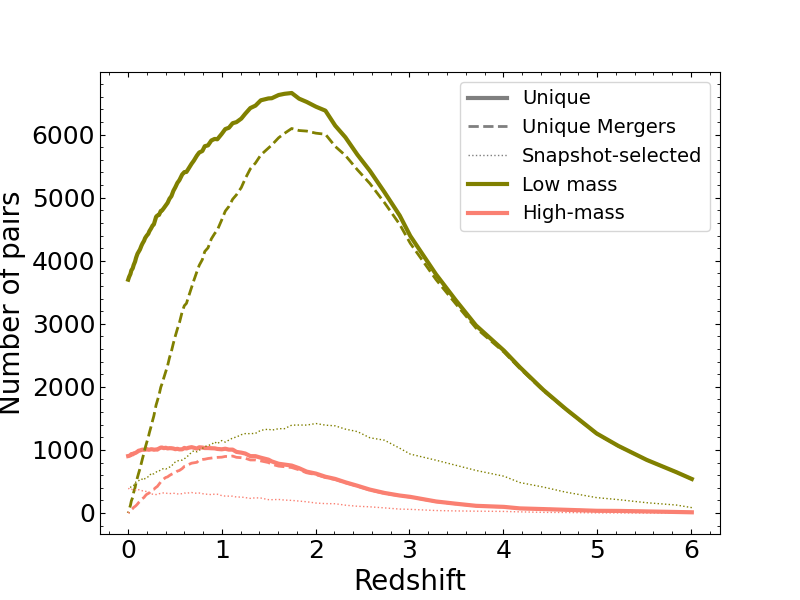
\includegraphics[width=\columnwidth]{plots/bet-on-it/6_paircount.png}
    \caption{The number of low-mass (green) and high-mass (pink) unique pairs (or distinct orbits) that are post-infall and pre-merger as a function of redshift. 
    The solid lines show the total number of pairs at a given redshift (including non-mergers and mergers that have yet to merge), while dashed lines show the number of post-infall orbits at a given redshift that will merge before $z=0$.
    We only count the number of orbits ``at" a given redshift if they have not merged, but have experienced first infall at a previous time (i.e. post-infall). 
    The decrease in the number of unique low-mass pairs from $z=2$ to $z=0$ is due to pairs being removed from the sample via mergers.
    }
    \label{fig:numorbits}
    \end{center}
\end{figure}

\begin{figure}[htb]
    \begin{center}
    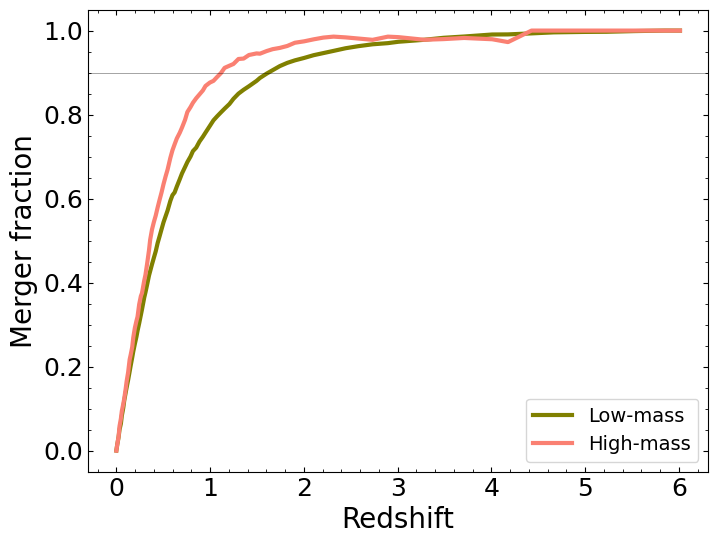
\includegraphics[width=\columnwidth]{plots/bet-on-it/6_mergerfraction.png}
    \caption{The fraction of low-mass (green) and high-mass (pink) post-infall orbits that result in a merger before z=0 as a function of redshift. 
    The horizontal line shows a merger fraction of 0.9, or 90\%. 
    High-mass pairs have merger fractions greater than 0.9 for $z>1.1$, and low-mass pairs for $z>1.6$.
    %At $z>1$, the fraction of selected pairs that merge before $z=0$ is upwards of 80\% for both low mass and high mass isolated pairs. 
    The sharp decline of the merger fraction to 0 at low redshift is a non-physical feature of the simulation ending at $z=0$.
    Only orbits with sufficiently short merger timescales will be able to merge at these redshifts.}
    \label{fig:fmerge}
    \end{center}
\end{figure}

\subsection{Number of Pairs}
We calculate the number of pairs by selecting all pairs at a given redshift that have not merged.
% The number of orbits that result in mergers at a later redshift are selected in the same way, excluding the non-merging orbits.
%For example, the total number of orbits at $z=2$ includes the orbits of pairs that passed the selection criteria at \textit{any} redshift, provided they achieved first infall at $z\geq2$ and have a merger redshift $z<2$. 
A single, non-merging pair with first infall at $z=3$ will thus contribute to the number of pairs at all redshifts from $z=0-3$. 

Figure~\ref{fig:numorbits} shows the number of low-mass and high-mass pairs as a function of redshift from $z=0-6$. 
Low-mass pairs (green solid line) are most numerous between $z=1.25-2$, while unique high-mass pairs (pink solid line) are most numerous between $z=0-1$.
The dashed lines show the number of unique pairs that merge prior to $z=0$ for each sample. 
The number of pairs that merge decreases to zero at $z=0$ since many pairs that exist at low redshift will have merger timescales that span beyond the end of the simulation (i.e., $z=0$). 

As more subhalos experience first infall into a FoF, the number of pairs increases with decreasing redshift. 
On the other hand, as mergers occur, the number of pairs decreases with decreasing redshift, as pairs that have merged are no longer members of the pairs sample.
% The difference between high and low mass
The number of low-mass pairs continues to increase from $z=6$ until around $z=2$, at which point the number of added pairs at a given redshift slows. 
The decrease in the number of pairs after $z=2$ means that the number of low-mass pairs that are merging at each redshift is larger than the rate at which pairs are being added to the sample.

The number of high-mass pairs continues increasing until $z=1$, at which point it remains approximately constant from $z=0-1$ at $\sim1000$ pairs. 
There is a slight decrease in the number of high mass pairs at the very lowest redshifts $z<0.1$, where the mergers begin to outnumber the new pairs being added at each redshift.

In Fig.~1 of \chambe{}, the number of low-mass pairs peaks (with $\sim3,000$ pairs) and begins to decrease at $z\sim2$, and the number of high-mass pairs is approximately constant between $z=0-1$, peaking at $\sim700$ pairs. 
We find the same behavior with our pair sample, with low-mass pairs peaking at z=2 and high mass pairs leveling off between $z=0-1$. 
However, in this study, the number of pairs at a given redshift is higher than in our previous work, since the orbit catalog includes a unique orbit for every pair from the previous work.
For example, a pair that passes the \chambe{} selection criteria only at $z=1$ will only be counted as a pair at $z=1$ in the previous work, while, in this study, it may be counted at many more redshifts since we can follow the orbit forwards and backwards in time. 


\subsection{Merger Fraction}
We calculate the merger fraction by dividing the number of pairs that merge (dashed lines in Fig.~\ref{fig:numorbits}) by the number of total unique orbits (solid lines) at a given redshift, including all pairs that do and do not merge. 
As before, an orbit with first infall at $z=2$ and merger at $z=1$ will be included in the merger fraction calculation for redshifts $z=1-2$.

Figure~\ref{fig:fmerge} shows the fraction of isolated pairs of low-mass (green) and high-mass (pink) pairs that merge before the end of the simulation as a function of redshift. 
At redshifts $z>2$, the merger fraction for low-mass and high-mass pairs is greater than $0.9$.
The merger fraction for both mass ranges declines to zero at $z=0$, due to the very low fraction of pairs at low redshift ($z<1$) that have short enough merger timescales to merge before $z=0$.

% difference/similiarity between low and high
The merger fraction of low-mass and high-mass pairs is the same from $z=0-0.5$ and $z>2.5$. 
Between $z=0.5-2.5$, the high-mass merger fraction is higher than the low-mass merger fraction, and the knee of the merger fraction occurs at a lower redshift.
This is likely because the number of low-mass pairs continues to increase before turning over and beginning to decrease at $z\sim2$, while the number of high-mass pairs continues increasing to $z\sim1$. 
At these redshifts, the number of merging pairs begins declining rapidly. 
% When the number of pairs stops increasing and beings to decrease, pairs that will not have time to merge before $z=0$ are being added, while many merging pairs are being removed from the sample, thus decreasing the merger fraction. 
Since the turnover for the number of high-mass pairs occurs at a lower redshift, the knee of the merger fraction is likewise shifted to lower redshifts.

Note that the merger fraction defined here is a measure of the fraction of isolated pairs that merge before $z=0$. It is not, however, a measure of the fraction of \textit{all} low-mass and high-mass pairs in all environments that will merge. 




% ###########################################################################################
% Results I
% ###########################################################################################
\begin{figure*}[htb]
    \begin{center}
    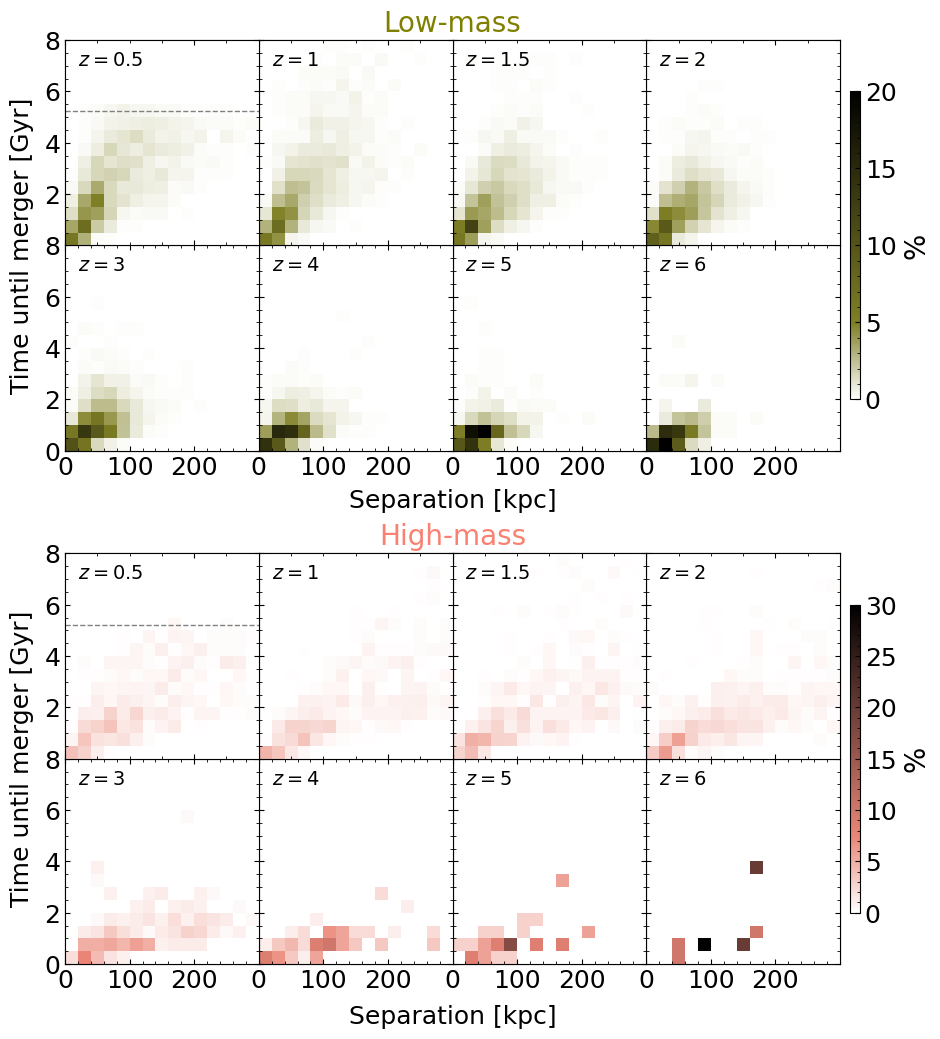
\includegraphics[width=0.8\textwidth]{plots/bet-on-it/8_2Dhist.png}
    \caption{\kc{(and add number of pairs at that redshift?) Add low/high label somewhere, is the lower sep set to 10kpc?} The distribution of times until merger for low-mass pairs as a function of physical separation at $z=0.5,1,1.5,2,3,\mbox{and }4$. 
    There is a positive correlation between separation at the selected redshift and the time until merger. 
    Of orbit-selected merging pairs at $z=1$, the majority are found with separations $\rsep<100\,\kpc$, and will merge within $3-4\, \Gyr$. 
    Merger times are longer for lower redshift pairs, and the distribution of separations is larger.
    The lowest separation pairs have the shortest merger timescales.
    This plot can be used to get estimates for the merger timescale of an isolated low-mass pair at a given redshift. For example, a low-mass pair at $z=2$ with $\rsep\sim 75\,\kpc$ will merge in $0-6\,\Gyr$, with a most likely time to merger of around $2\Gyr$.
    \kc{add z=5, z=6, add horizontal line for the time remaining in the sim in panel 1}
    }
    \label{fig:timevssep-low}
    \end{center}
\end{figure*}

\begin{figure*}[htb]
    \begin{center}
    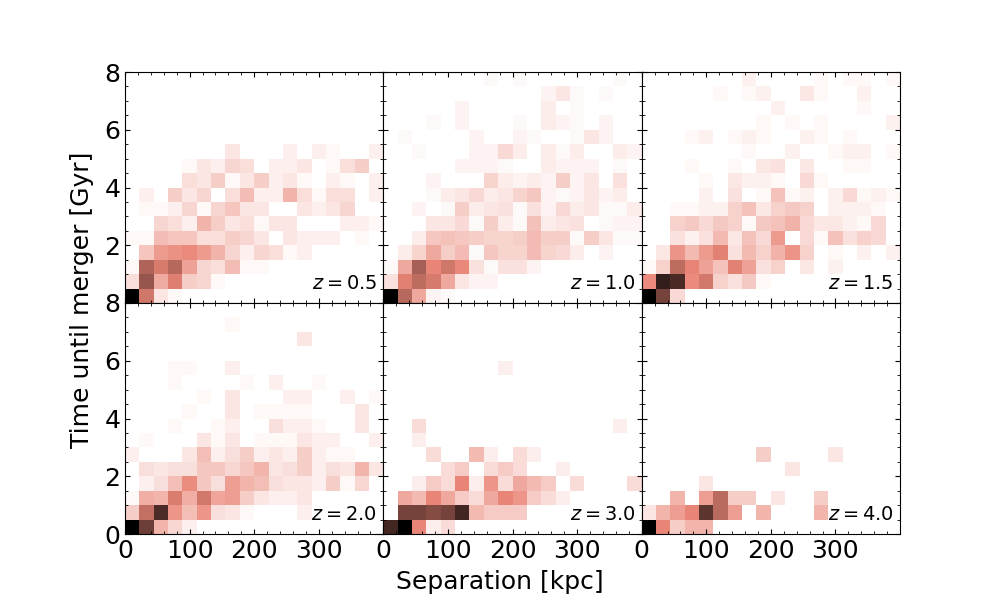
\includegraphics[width=0.7\textwidth]{plots/bet-on-it/3_Timevssephigh-2d.png}
    \caption{\kc{Add z=5, z=6 panels. Add colorbar. Add low/high label somewhere, check the lower sep set to 10kpc?} The distribution of times until merger for high-mass pairs as a function of physical separation at $z=0.5,1,1.5,2,3,\mbox{and }4$.
    Similar to the low-mass pairs, there is a positive correlation between the separation of a merging pair at a given redshift and the time until merger, with the lowest separation pairs tending to have the shortest time until merger.
    Of orbit-selected merging pairs at $z=1$, the majority are found with separations $\rsep<200\,\kpc$, and will merge within $0-7\, \Gyr$. 
    This plot can be used to get estimates for the merger timescale of an isolated high-mass pair at a given redshift. 
    For example, a high-mass pair at $z=2$ with $\rsep\sim 150\,\kpc$ will merge in $0.5-4\,\Gyr$, with a most likely time to merger of around $1.5-2\Gyr$.
    }
    \label{fig:timevssep-high}
    \end{center}
\end{figure*}

\section{Results: The Mass and Redshift Dependence of Merger Timescales}
    Using our sample of isolated low-mass and high-mass pairs in the TNG100 simulation, we calculate the merger timescales, or time until merger, for all of the merging pairs in our catalog. 
    The merger timescale of a pair is defined to be the amount of time that elapses in the simulation between the selected redshift and the merger redshift.\footnote{Since our orbits are only defined for a pair post-infall, the merger timescales will likewise only be calculated for pairs that are post-infall at the given separation.}
    
    In Sec.~\ref{sec:results-timevsep}, we explore how the merger timescale changes as a function of the separation of the pair across redshifts, and how the merger timescales differ between the low-mass and high-mass pairs. 
    In Sec.~\ref{sec:results-timevredshift}, we investigate the median time until merger for all post-infall and pre-merger isolated pairs as a function of redshift. 
    We will additionally examine the merger timescale's dependence on a variety of separation criteria. 
    Separation criteria are applied to pairs at each redshift independently, such that a pair in the $10-50\,\kpc$ bin at one redshift will not be part of the sample used at redshifts where its separation is $>50\,\kpc$.




\subsection{Separation Dependence of Merger Timescales}\label{sec:results-timevsep}
    % how we calculate for this section
    We calculate the time until merger as a function of separation for low-mass and high-mass pairs at a variety of redshifts from $z=0.5-6$. 
    % Pairs with small separations may be undergoing a pericentric passage, or very close to merging if on a radial orbit.
    Binning the pairs by separation, we can study how the merger timescale changes for pairs at different points in their orbits. 
    
    % low mass example
    We bin our pair sample by merger timescale, in bins of $0.5\Gyr$, and separation bins of $10\,\kpc$.
    Figures~\ref{fig:timevssep-low} and~\ref{fig:timevssep-high} show the 2D distributions of merger timescale vs. separation for low-mass and high-mass pairs at redshifts $z=(0.5,1,1.5,2,3,4,5,6)$. 
    The horizontal line in the first panel shows the time remaining in the simulation until $z=0$, above which no merging pairs exist. \kc{add to fig.}
    
    Fig.~\ref{fig:timevssep-low} presents a heatmap distribution of the density of low-mass pairs in merger timescale-separation space. 
    We find that the time until merger for low-mass pairs is positively correlated with the separation of the pair at each redshift. 
    However, the slope of the correlation decreases at higher redshifts.
    Pairs at $z=4$ and separations between $50-100\,\kpc$ tend to merge in less time than pairs with the same separations at $z=0.5$. 
    
    In addition, the spread of times until merger and separations is smaller at higher redshift. 
    The spread of merger timescales at $z=1$ goes from $0-8\,\Gyr$, while pairs at $z=4$ have merger timescales between $0-3\,\Gyr$. 
    Likewise, the spread of separations at $z=1$ is $0-200\kpc$, but at $z=4$ the spread is smaller, between $10-125\kpc$. 
    This is due to the growth of halos over time, such that more pairs are identified at low redshifts where the virial radius of FoF groups is larger. 
    
    Likewise, Fig.~\ref{fig:timevssep-high} presents the distribution for high-mass pairs.
    The trends between merger timescale and separation are roughly the same as low-mass pairs, with a positive correlation between the two parameters that decreases in slope from low redshift to high redshift. 
    The high-mass pairs also have a larger spread in the distribution of merger timescales and separations at low redshift than at higher redshift.
    This is once again caused by the change in the FoF halo size over time. 
    
    % 
    \begin{table*}[]
\centering
\begin{tabular}{c|c|c|c|c|c|c|c|c|c}
\hline \hline
\multirow{2}{*}{Redshift} & Separation & Total \# & \multicolumn{7}{c}{Time Until Merger} \\ \cline{4-10}
 & [kpc] &  of Orbits & $0-0.5\,\Gyr$ & $0.5-1\,\Gyr$ & $1-1.5\,\Gyr$ & $1.5-2\,\Gyr$ & $2-2.5\,\Gyr$ & $2.5-3\,\Gyr$ & $3+\,\Gyr$  \\ \hline
\multirow{6}{*}{z=1} & 10-50 &  &  &  &  &  &  &  &  \\
 & 10-75 &  &  &  &  &  &  &  &  \\
 & 10-100 &  &  &  &  &  &  &  &  \\
 & 10-150 &  &  &  &  &  &  &  & \\
 & 10-200 &  &  &  &  &  &  &  & \\
 & 10-300 &  &  &  &  &  &  &  & \\  \hline 
 \multirow{6}{*}{z=2} & 10-50 &  &  &  &  &  &  &  &  \\
 & 10-75 &  &  &  &  &  &  &  &  \\
 & 10-100 &  &  &  &  &  &  &  &  \\
 & 10-150 &  &  &  &  &  &  &  & \\
 & 10-200 &  &  &  &  &  &  &  & \\
 & 10-300 &  &  &  &  &  &  &  & \\ 
 \hline \hline
\end{tabular}
\end{table*}
    A compilation of more specific data is available in Table~\ref{tab:timevssepvsz}.
    Here, we list the fraction of pairs within three separation bins $(10-50, 10-70, 10-100)\,\kpc$, and the fraction of pairs within each of those separation bins that merge in four different timescale bins $(0-1, 1-2, 2-3, 3+)\,\Gyr$.
    We present these data for redshifts of $z=(0.5,1,1.5,2,3,4,5,6)$.
    
    Data from the table can be interpreted in the following way: at $z=1.5$, there are 5,787 pairs that are post-infall and merge prior to $z=0$. 
    Of those, 2,458 (42.47\%) have low separations between $\rsep=10-50\,\kpc$, and 2,207 of those $10-50\,\kpc$ pairs will merge in the next $2\,\Gyr$. 
    
    \begin{figure}[htb]
        \centering
        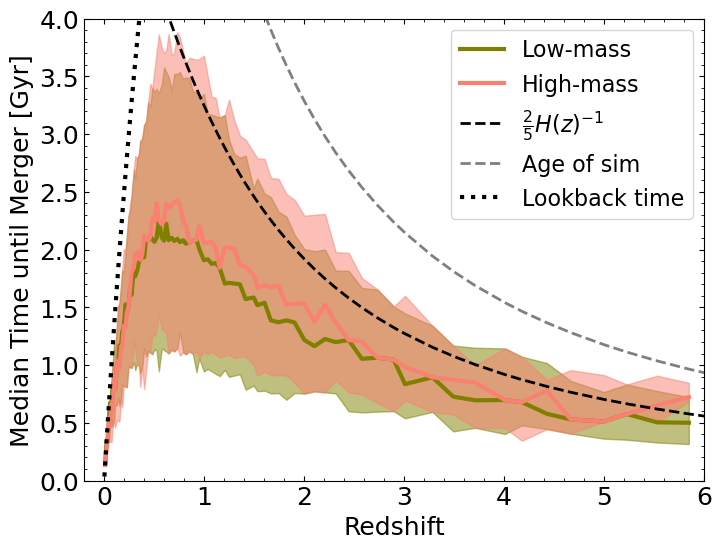
\includegraphics[width=\columnwidth]{plots/bet-on-it/8_timescale_mod.png}
        \caption{The median time until merger as a function of redshift for low-mass (green) and high-mass (pink) pairs. Shaded regions represent the 1st and 3rd quartile spread on the median. Pairs at each redshift are selected if they have experienced first infall and are pre-merger. 
        % 
        The black dashed line shows a fraction of the Hubble time as a function of redshift, which bounds the median time until merger from $z=6$ to $z\sim0.5-0.75$.
        The dotted black line shows the time to $z=0$ (the lookback time) as a function of redshift, which sets the upper bound for the time until merger that a merging pair can have. 
        The median time until merger is similar for low-mass and high-mass pairs, and rises from $z=6$ to a peak at $z\sim0.75$, then decreases to $z=0$.\kc{only one of the dashed lines will remain in this plot once I discuss w Paul}}
        \label{fig:timescales}
    \end{figure}
    
    \begin{figure*}[htb]
        \centering
        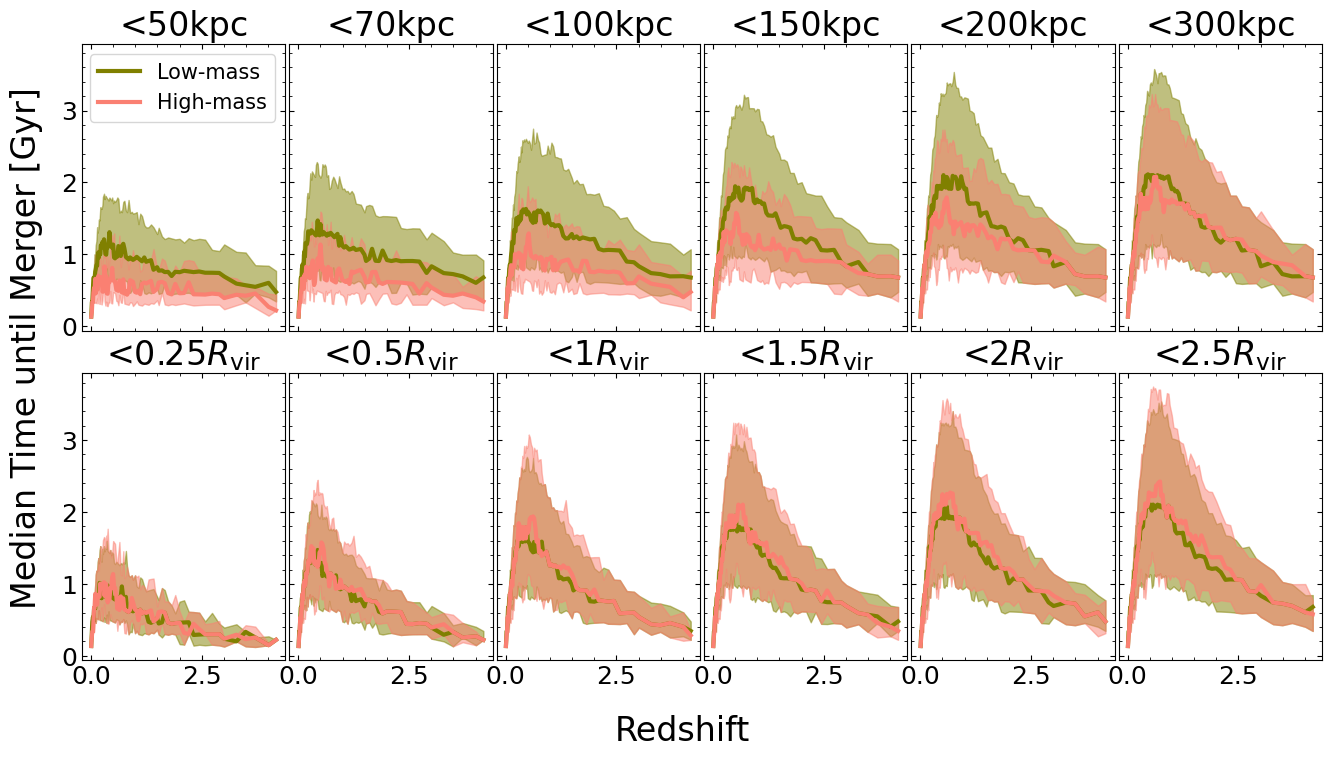
\includegraphics[width=\textwidth]{plots/bet-on-it/3_time_til_merger.png}
        \caption{(Top) The median time until merger as a function of redshift for low-mass (green) and high-mass (pink) pairs with 3D physical separations greater than $10\,\kpc$ and less than $(50,70,100,150,200,\mbox{and }300)\,\kpc$ from left to right. 
        (Bottom) The median time until merger as a function of redshift for pairs with physical separations greater than $10\,\kpc$ and less than $(0.25, 0.5, 1, 1.5, 2,\mbox{and }2.5)\,\Rvir$ from left to right. 
        % 
        The time until merger increases from $z=4$ to $z\sim0.5-0.75$, at which point the time until merger decreases to zero since all low redshift mergers must have short merger timescales to merge before the end of the simulation at $z=0$. 
        }
        \label{fig:timescales-sep}
    \end{figure*} 
    
\subsection{Redshift Dependence of Merger Timescales}\label{sec:results-timevredshift}
    % The behavior of time until merger as a function of redshift for low-mass and high-mass pairs:
    % 1 - the full sample 
    % 2 - the physical and static kpc separation-selected sample
    % 3 - the mass and redshift evolving scaled separation-selected sample
    In this subsection, we study the merger timescale of low-mass and high-mass pairs as a function of redshift. 
    
    First, we consider the pairs sample as a whole, and quantify the median merger timescale for all low- and high-mass pairs that are post-infall and pre-merger for $z=0-6$. 
    We will then consider two different sets of separation criteria to create separation-selected subsamples.
    Since pair samples are typically picked via separation criteria, in both simulations and observations, we study the impact of different separation-based selection criteria on inferred merger timescales.
    
    Each merging orbit is defined to start at first infall, and 
    


    \subsubsection{Full sample}
        We calculate the merger timescales for pairs at each redshift in the simulation from $z=0-6$, and quantify the median and spread on the merger timescale as a function of redshift. 
        We include the full catalog of merging orbits at each redshift to calculate the merger timescale. 
        % why do we want to consider the entire population of halos? why interesting?
        
        Figure~\ref{fig:timescales} presents the median of the time until merger for post-infall merging pairs from $z=0-6$. 
        The 1st and 3rd quartiles are indicated with shaded regions. 
        % low vs high
        Low-mass merger timescales (green) and high-mass merger timescales (pink) are roughly equivalent at all redshifts, which implies that mergers do not proceed in fundamentally different ways at different mass scales. 
        We explore this point further in Sections~\ref{sec:results-phys} and~\ref{sec:results-scal}.
        
        % redshift evolution
        The median time until merger is $\sim0.5-0.7\,\Gyr$ at $z\sim6$, then rises to a peak of $2.3-2.4\,\Gyr$ at $z\sim0.6$, then decreases to 0 at $z=0$.
        The abrupt decrease to 0 from $z\sim0.6$ to $z=0$ is artificial rather than a true physical feature. 
        As $z\to0$, there is an increasingly small fraction of pairs that merge before $z=0$, as seen by the dashed lines in Fig~\ref{fig:numorbits}. 
        These mergers must then proceed on timescales less than the elapsed time difference between a given redshift and $z=0$. 
        This is shown by the dotted black line on the left of Fig.~\ref{fig:timescales}, which shows the lookback time of the simulation as a function of redshift.\footnote{The lookback time at a given redshift $z_n$ is equivalent to the time elapsed between $z_n$ and $z=0$. Thus, merging pairs cannot have merger timescales larger than the lookback time of the simulation at a given redshift.} % this could go in the methods section, if we think it's more necessary there. I don't mind it here for more detail

    % this is all really discussion, so I can either move this to discussion and reference that we talk about the H(z) line more explicitly in the discussion, or not
        In principle, merger timescales\footnote{Specifically, the elapsed time between crossing into the virial radius of a subhalo and coalescence with the central galaxy.} for a body moving through a homogeneous field of collision-less matter can be analytically derived from the Chandrasekhar formula for dynamical friction~\citep{Binney2008}. 
        Departures from the idealized case introduce perturbations to that solution, the validity of which has been tested in cosmological hydrodynamic and N-body simulations~\citep{Jiang2008, Boylan_kolchin2008}. 

        Such studies have found that the merger timescale in N-body hydrodynamic simulations is of the form
        \begin{equation}
            \rm \tau_{\rm merge} = \frac{A(\Theta)}{\ln \Lambda}\frac{\mprim}{\msec}\tau_{\rm dyn}
        \end{equation}
        where $\mprim$ and $\msec$ are the primary and secondary subhalo masses, $A(\Theta)$ is a constant for a given orbital configuration, $\ln\Lambda$ is the Coulomb logarithm taken to be $\ln\Lambda = \ln(1+\mprim/\msec)$, and $\tau_{\rm dyn}$ is the dynamical timescale at the virial radius of the primary subhalo.
        The dynamical timescale is related to the crossing time at the virial radius, and is given by 
        \begin{equation}
            \rm \tau_{\rm dyn} = \frac{\Rvir}{V_{\rm circ}(\Rvir)},
        \end{equation}
        where $V_{\rm circ}(\Rvir)$ is the circular velocity at the virial radius of the primary subhalo. 
        Note that the dynamical time can be rewritten as 
        \begin{equation}
            \rm \tau_{\rm dyn} = (G\rho_{crit})^{-1/2} = \bigg(\frac{3\,H^2(z)}{8\pi}\bigg)^{-1/2}.
        \end{equation}

        In our study, we keep the stellar and FoF group mass criteria fixed as a function of redshift, such that for a given pair, the merger timescale scales with redshift as
        \begin{equation}
            \rm \tau_{merge} \propto \tau_{dyn} \propto H(z)^{-1},
        \end{equation}
        assuming that there is no (or weak) redshift dependence of the distribution of orbital parameters.
        Thus, the merger timescale is expected to scale with the Hubble Time at a given redshift. 
        
        In Fig.~\ref{fig:timescales}, the black dashed line represents a merger timescale that scales with $1/H(z)$,
        \footnote{$H(z)$ is calculated using the same cosmology as the TNG100 simulation. Specifically, $\Omega_M=0.31$ and $\Omega_{\Lambda}=0.69$.}
        and which is consistent with our findings for redshifts between $z=1.5-6$. 
            

    \subsubsection{Physical Separation Selected Pairs }
    \label{sec:results-phys}
        Both separation selected samples have a lower separation criteria of $10\,\kpc$, to limit the impact of subhalos becoming indistinguishable in the \subfind{} catalogs.
        This lower separation criteria is also commonly applied to observationally selected pairs in studies of merger fractions and merger rates (see Sec.~\ref{sec:discussion} for further detail).
        
        The first set of separation criteria will select only pairs at a given redshift that have separations greater than $10\,\kpc$ and less than $[50, 70, 100, 150, 200, \mbox{and }300]\kpc$, dividing the sample into six pair subsamples. 
        These separation criteria do not vary as a function of time or mass, and are applied equivalently to the low-mass and high-mass samples at all redshifts. 
        We note that an orbit in the separation bin $10-50\,\kpc$ at $z=2$ will not necessarily be in that same bin at other redshifts. 
        Rather, the separation criteria are applied independently at each redshift. 
        
        % figure description 
        The top panel of Fig.~\ref{fig:timescales-sep} shows the time until merger versus redshift for each of the low-mass (green) and high-mass (pink) pair subsamples with separations less than the physical separation listed above each column.  
        % redshift evolution of each subsample
        We first note that the merger timescale peaks around redshift $z\sim0.5$ for all low-mass and high-mass subsamples. 
        In addition, all subsamples show the same decline of mean merger time as $z\to0$, as discussed in the previous section. 
        These traits were also present in Fig.~\ref{fig:timescales}, so they are features that are roughly independent of a separation criteria.
        As the selection criteria gets larger, the subsample contains more of the full sample, eventually including the full sample at large enough separations.
        
        % low mass vs high mass
        The subsamples with maximum separations of $[50, 70, \mbox{and } 100]\,\kpc$ result in median merger timescales that are higher for low-mass pairs than high-mass pairs at all redshifts. 
        The difference in the median time until merger is up to $0.8\,\Gyr$ longer for low-mass pairs than high-mass pairs at the same redshift for the same separation criteria. 
        The offset between the low-mass and high-mass merger timescale decreases for each successive separation cut, which will each include pairs with larger separation. 
        In the rightmost top panel, the median merger times overlap almost identically for $z=0-0.5$ and $z>1.5$, almost mimicking our findings from the full sample analysis. 
        
        % impact of the separation criteria
        When the maximum separation is increased (from left to right), more of the full sample is used in the calculation for the median merger timescale. 
        Indeed, the merger timescale for both low-mass and high-mass pairs increases with an increasing maximum separation cut.  
        This follows directly from Sec.~\ref{sec:results-timevsep}, where we found that the time until merger is positively correlated with increasing separation for all pairs. 
        Thus, including a higher fraction of larger-separation systems in our merger time calculation tends to increase the median time until merger. 
        
        The median merger timescale for low-mass pairs does not change significantly for any separation criteria $>150\,\kpc$. 
        On the other hand, high-mass pairs tend to see an increase in the merger timescale for each larger separation cut. 
        This is because selecting all pairs with $\rsep<200\,\kpc$ in a low-mass system is including a larger volume of the FoF halo, and thus a more complete selection of the full sample.
        High-mass pairs tend to have higher separations than low-mass pairs, as shown in~\ref{sec:results-timevsep}. 

    \subsubsection{Scaled Separation Selected Pairs}
    \label{sec:results-scal}
        We calculate the merger timescales for six additional subsamples of pairs, this time applying separation criteria that scale with both redshift and mass.
        The scaled separation, which we define in Section~\ref{sec:methods}, is the separation of a pair divided by the virial radius of the pair's FoF group, $\Rvir$. 
        The scaled separation selected pairs have separations greater than $10\,\kpc$ and less than $<[0.25, 0.5, 1, 1.5, 2, 2.5]\,\Rvir$. 
        As in the previous section, the selection criteria are applied at each redshift independently. 
        
        As detailed in \chambe{}, the median virial radius for low-mass FoF groups at $z=[0,1,2,3,4]$ is approximately $[134, 85, 59, 43, 33]\,\kpc$, and for high-mass FoF groups is approximately $[348, 206, 134, 97, 76]\,\kpc$.
        Thus, choosing a scaled separation cut of $<1\,\Rvir$ at $z=1$ will select high-mass pairs with separations $\lesssim205\,\kpc$ and low-mass pairs with separations $\lesssim85\,\kpc$.
        
        % figure description 
        The bottom panel of Fig.~\ref{fig:timescales-sep} shows the median time until merger versus redshift for low-mass (green) and high-mass (pink) pair subsamples with scaled separations less than those listed at the top of each plot. 
        We find that the median time until merger at $z=1$ is $[0.64, 0.94,1.25,1.51-1.58,1.76-1.91,1.91-2.05]\,\Gyr$ for each scaled separation cut respectively, for both low-mass and high-mass samples. %\kc{gonna have to triple check this cause I get the SAME median time til merger for low and high mass for Rvir 0.25, 0.5, and 1, down to like 14 decimals...}
        
        % redshift evolution of each subsample
        Similar to the static physical separation-selected subsamples in the top panel, the median time until merger starts off small at $z>4$, then increases to a peak around $z\sim0.5$, before quickly decreasing to 0 at $z=0$. 
        Additionally, the median time until merger at a given redshift increases for separation criteria that include a larger fraction of the virial radius, and thus larger separation pairs. 
        
        % low mass vs high mass
        However, quite unlike the physical separation selected subsamples in the top panels, using a scaled separation criteria results in nearly identical median merger timescales for low-mass and high-mass pairs at all redshifts.
        The low-mass and high-mass merger timescales increase with each larger scaled separation cut, but recover the behavior of the full sample by $<2\,\Rvir$.
        
        In addition, the slope of the time until merger as a function of redshift for $z>0.5$ is steeper for high-mass pairs in the scaled separation subsamples than the physical separation subsamples.
        This is especially noticeable in the first panel of both the top and bottom rows, where the merger timescale of high-mass pairs is approximately flat for $<50\,\kpc$. 
    
    

% ##################
% Discussion section
\section{Discussion} \label{sec:discussion}
    We have calculated the merger timescales, or time until merger, for a sample of low-mass and high-mass pairs that have experienced first infall but not yet merged, to ensure that they are physically collocated.
    In this section, we will explore the implications and broader impacts of our findings, and put our study in context with previous work. 
    %In Sec.~\ref{}, etc...
    
    \begin{itemize}
        % \item Implications for 
        \item Sec 1: Comparison to previous works: merger fraction/timescale studies
        %Why did we pick the separation cuts that we did? 
        \begin{itemize} 
            \item What other studies have looked at merger fractions/timescales in hydro simulations, specifically? 
            \item Have they studied merger fractions as a function of mass and redshift? What did they find?
            \item Were low-mass pairs expected to have such high merger rates in isolated environments? 
            \item Have they studied merger timescales as a function of mass and redshift? 
            \item What is unique about our study?
            \item Are comparisons with previous works fair, or are they not really comparable?
            \item specific papers: Ventou 2017, Hopkins 2007, O'Leary 20
        \end{itemize}

        \item Sec. 2: Implications for observational merger fractions and merger rates
        \begin{itemize}
            \item How did we motivate separation criteria?(motivated already in Chambe+ 2024, restate here about close pair definitions from lit.)
            \item Pair fractions can vary wildly depending on separation criteria
            \item This is important too for merger rates, since they are a function of pair fractions and merger timescales, and you should really be selecting pairs at each stage as self-consistently as possible
            \item What is our suggestion moving forwards?
            \item specific papers: Lotz 2011, 
        \end{itemize}
        \item Sec 3: The functional form of the merger timescale
        \begin{itemize}
            \item What can we say about the fact that the merger timescales follow a $(1+z)^{-1}$ relation at $z>0.5-1$? Physical explanation for this behaviour? 
            \item Scaled separation criteria are akin to picking the same fraction of the total volume of a FoF group, regardless of what redshift it is at, not what mass it has, so it may not be surprising that we got what we did in re: the scaled separation being better, but finding the SAME merger timescales for hi and low is interesting!
            \item Maybe something to consider in this section: For things that don't merge, what's... going on? 
            \item relevant papers: 
        \end{itemize}
    \end{itemize}
    
    Bring up assumption of isolation criteria and it's drawbacks and strengths.
    Reiterate that our findings are for isolated pairs. 
    
    
    
\section{Summary and Conclusions}
    % what we did and how
    $<$Longer summary of what we did here$>$
    
    % set of conclusions from results
    Our main findings are as follows: 
    \begin{itemize}
        \item for a given physical separation (such as 100kpc), high-mass pairs have shorter merger timescales than low-mass pairs. 
        \item the median time until merger for the full sample of low and high-mass pairs increases as $\sim(1+z)^{-1}$ from $z=6$ to $z\sim0.75$. it then decreases to 0 at low redshifts, with an upper bound set by the time remaining in the simulation before $z=0$. The decrease in the merger time at low redshifts is artificial and not representative of the true merger timescales that pairs at $z=0$ will have.
        \item separation criteria that include larger separations will increase the median time until merger.
        \item static physical separation-selected subsamples of low- and high-mass pairs have different median merger timescales.
        \item scaled separation-selected subsamples yield nearly identical median merger timescales for low-mass and high-mass pairs at all redshifts. 
    \end{itemize}
    
    % set of conclusions for discussion
    - We find that the merger timescale of low-mass or high-mass merging pairs is sensitive to the selection criteria that are used to define the pair sample.\\
    
    - We recommend that future studies that seek to compare or compute pair fractions, merger fractions, merger timescales, or merger rates, define selected pair samples using separation criteria that evolve with redshift and mass. 
    
    - Why is this important? Cause future studies are gonna get so many pairs, especially low mass, and now we have a framework to compare low and high mass pairs in a variety of ways, from pair fractions to merger fractions to merger timescales! Woo!
    
    Further work that would be nice to do would be to see if all the timescale stuff stays the same for minor mergers, and for smaller bins in range 1-1:4


% ** 
% \appendix
% adfadfa








\bibliography{refs}{}
\bibliographystyle{aasjournal}

\end{document}

